%xelatex
\documentclass[12pt]{article}

\usepackage[T2A]{fontenc}
\usepackage[english,ukrainian]{babel}
\usepackage{fontspec}
\setmainfont{Nimbus Roman}
\usepackage{newtxmath}
\usepackage{gensymb}
\usepackage{graphicx}
\usepackage[a4paper,margin=0.5in]{geometry}
\pagestyle{empty}

\usepackage{pgfplots}% loads the package tikz
\pgfplotsset{compat=1.18}
\usetikzlibrary{intersections}
\usepackage{wrapfig}
\usepackage{indentfirst}
\usepackage{pdfpages}
\usepackage{subfiles}

\begin{document}
\includepdf[pages=-]{35tit.pdf}
{\fontsize{14}{16.2}\selectfont

\subsection*{Мета роботи}
Ознайомитись з явищами обертання площини поляризації світла оптично
активними речовинами і штучного обертання площини поляризації світла
магнітним полем, а також визначити концентрацію цукру ряду розчинів

\subsection*{Прилади та обладнання}
Цукрометр типу СУ-4, набір трубок з розчинами цукру різних
концентрацій, соленоїд, випрямляч струму типу ВС-24М

\subsection*{Теоретичні відомості та опис установки}
В даній лабораторній роботі для вивчення явища обертання площини
поляризації світла використовується цукрометр типу СУ–4. Його
оптична схема наведена на рис. 1. Світло від лампи 1 проходить
через лінзу L, поляризатор 2, трубку з досліджуваним розчином 3,
компенсатор 4 та аналізатор 5. Поля порівняння світлових променів
спостерігають в окулярі 6 цукрометра.

\begin{figure}[h]
	\centering
	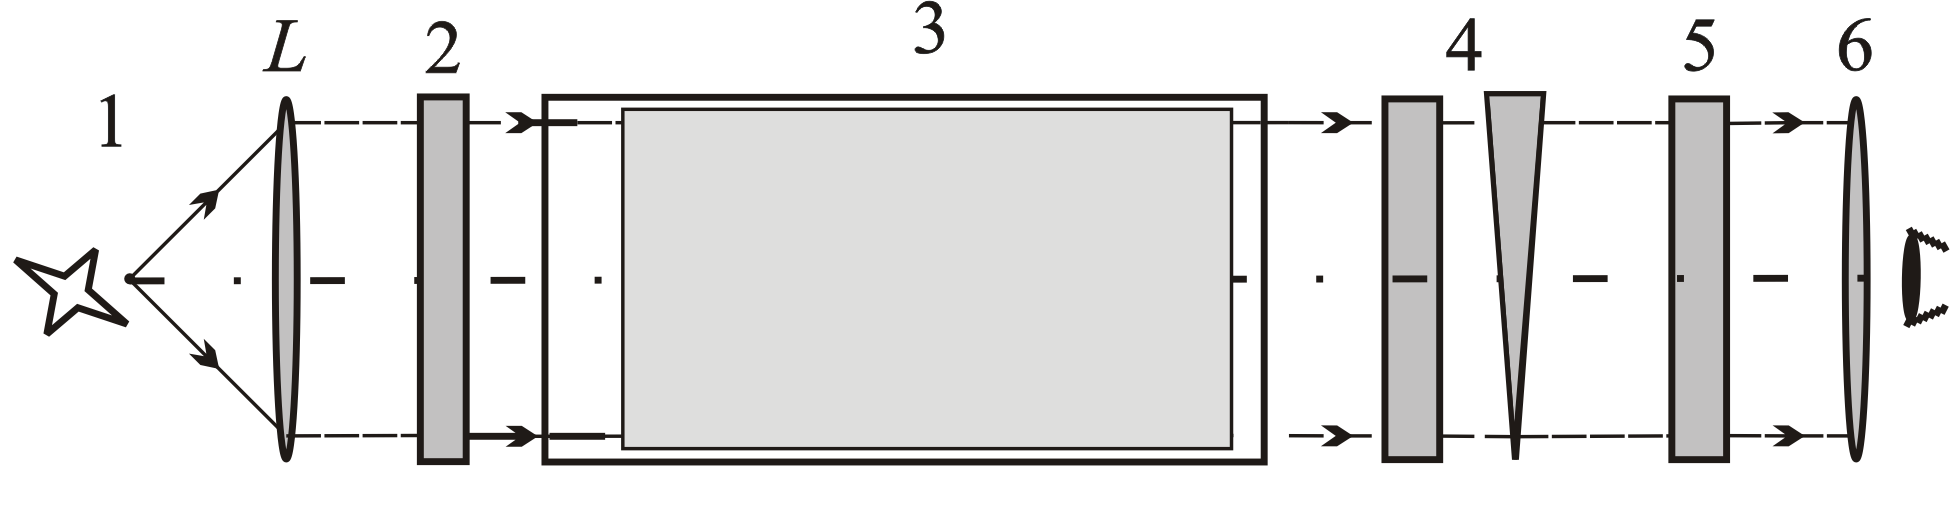
\includegraphics[width=.5\textwidth]{lens.png}
	\caption{оптична схема цукрометра}
\end{figure}

Зовнішній вигляд установки наведено на рис. 2.

\begin{figure}[h]
	\centering
	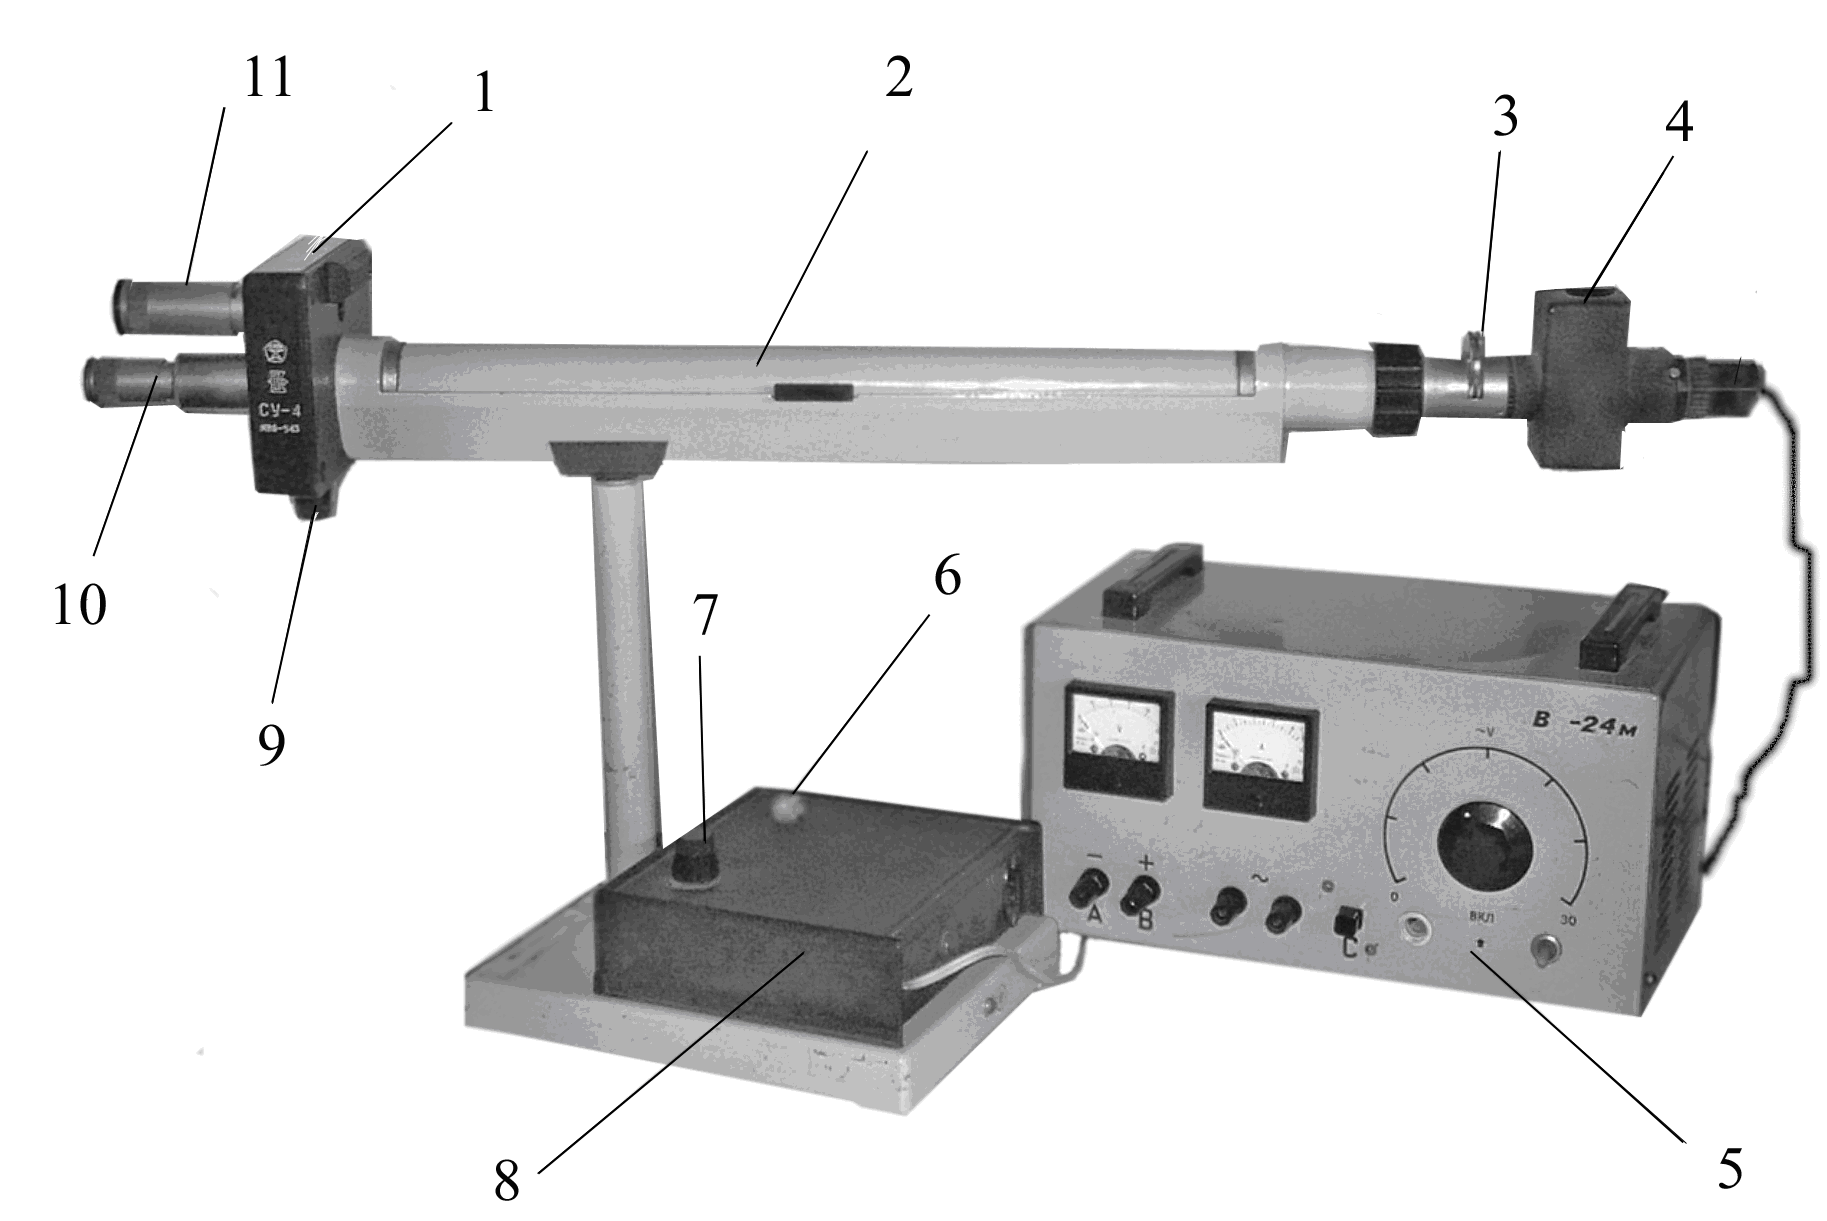
\includegraphics[width=.5\textwidth]{cukr.png}
	\caption{1 – вимірний вузол; 2 – кюветне відділення; 3 – тримач світлофільтрів; 4 – освітлювач, в якій знаходиться лампочка, лінза і поляризатор; 5 – випрямляч ВС–24; 6 – кнопка–вимикач; 7– регулятор яскравості освітлювача; 8 – блок живлення освітлювача; 9 – регулятор переміщення відлікової шкали і вирівнювання яскравості полів порівняння; 10 – зорова труба для спостереження полів порівняння світлових променів; 11 – зорова труба відлікової шкали.}
\end{figure}

В цукрометрі використовують міжнародну цукрову S – шкалу, за якою 100
поділкам відповідає 34,62$^\circ$. Відлік значень кута обертання площини
поляризації світла здійснюється за шкалою і ноніусом. Ціна поділки
ноніуса становить 0,05\textdegree S. До числа градусів, відрахованих за шкалою,
додають відлік за ноніусом.

Соленоїд живиться від випрямляча струму ВС-24М, на передній панелі
якого розміщені регулятор струму, кнопка для замикання електричного
кола, вольтметр і амперметр.

\subsection*{Задані величини}
Довжина кювети~--- 20 см, довжина соленоїда~--- 40 см, концентрація
розчину 1~--- $C_1=3.03\%.$

\subsection*{Фізичні величини, які вимірюються прямим способом}
відліки $n_i$ кутів обертання площини поляризації світла.

\subsection*{\centering{Таблиця результатів вимірювань}}

\renewcommand{\arraystretch}{1.3}
\begin{center}
	\begin{tabular}{|p{20pt}|p{25pt}|p{25pt}|p{25pt}|c|c|p{40pt}|p{30pt}|c|c|p{30pt}|p{30pt}|c|c|}
	\hline
		\No{} з/п & $\pm\bar n_0,$ \textdegree$S$ & \multicolumn{4}{c|}{Розчин 1}
		& \multicolumn{4}{c|}{Розчин 2} & \multicolumn{4}{c|}{Розчин 3} \\
	\cline{3-14}
		& & $n_1$, \textdegree$S$ & $\theta_1$, \textdegree$S$ & $\phi_1^\circ$ & $[\alpha]$ &
		$n_2$, \textdegree$S$ & $\theta_2$, \textdegree$S$ & $\phi_2^\circ$ & $C_2$ &
		$n_3$, \textdegree$S$ & $\theta_3$, \textdegree$S$ & $\phi_3^\circ$ & $C_3$ \\
		\hline
		1 & 0.75 & 8.35 & 7.73 & 2.7 & & -12.1 & -12.7 & -4.4 & & -1.2 & -1.82 & -0.6 & \\
		\cline{1-5} \cline{7-9} \cline{11-13}
		2 & 0.50 & 11.5 & 10.8 & 3.8 & 5.33 & -9.5 & -10.1 & -3.3 & 3.75 & -0.9 & -1.52 & -0.5 & 0.46 \\
		\cline{1-5} \cline{7-9} \cline{11-13}
		3 & 0.60 & 9.75 & 9.13 & 3.2 & & -12.2 & -12.8 & -4.4 & & -0.6 & -1.22 & -0.4 & \\
		\cline{1-5} \cline{7-9} \cline{11-13}
		сер. & 0.62 & 9.90 & 9.24 & 3.23 & & -11.26 & -11.8 & -4 & & -0.9 & -1.52 & -0.5 & \\
		\hline
%\textdegree$S$
\end{tabular}

\end{center}
}

\begin{center}

\subsection*{Обчислення шуканих величин за робочими формулами}
	\begin{equation}
		\theta_i=n_i-(\pm n_0)
	\end{equation}
	\begin{equation}
		[\alpha]=\frac{\phi_1}{C_1l}=\frac{3.23}{3.03\cdot0.2}=5.33
	\end{equation}
	\begin{equation}
		C_{2_\text{сер}}=\frac{\phi_2}{[\alpha]l}=\frac{4}{5.33\cdot0.2}=3.75~[\%]
	\end{equation}
	\begin{equation}
		C_{3_\text{сер}}=\frac{\phi_3}{[\alpha]l}=\frac{0.5}{5.33\cdot0.2}=0.46~[\%]
	\end{equation}

\subsection*{Обчислення похибок}
%	$\Delta n_1=\sqrt{1.1+0.025}=1.06$
	%$\sqrt{1.1+0,025}=1.06$
	\begin{align}
%	\Delta \theta_{1_\text{сер}}=(1.51+1.56+0.11)/3=1.06\\
	\Delta \theta_1=\sqrt{1.06+0.025}=1.0416,~
	\Delta \phi_1=0.3462\cdot 1.0416=0.3606~[^\circ]\\
	\Delta \theta_2=\sqrt{1.2+0.025}=1.1067,~
	\Delta \phi_2=0.3462\cdot 1.1067=0.3831~[^\circ]\\
	\Delta \theta_3=\sqrt{0.6+0.025}=0.7905,~
	\Delta \phi_3=0.3462\cdot 1.7905=0.2736~[^\circ]
	\end{align}

\begin{equation}
	\begin{aligned}
	\delta [\alpha]=\ln{\phi_1}-\ln C_1-\ln l=\\
	\frac{d\phi_1}{\phi_1}-\frac{dC_1}{C_1}-\frac{dl}{l}=
	\frac{\Delta\phi_1}{\phi_1}+\frac{\Delta C_1}{C_1}+\frac{\Delta l}{l}=\\
	\frac{0.3606}{3.23}+\frac{0.005}{3.03}+\frac{0.05}{0.2}=0.3632~[\%]
	\end{aligned}
\end{equation}
\begin{equation}
	\Delta [\alpha]=5.33\cdot 1.3632/100=0.01935
\end{equation}

\begin{equation}
	\begin{aligned}
		\delta C_2=\ln\phi_2-\ln[\alpha]-\ln l=\frac{d \phi_2}{\phi_2}
		-\frac{d \alpha}{\alpha}
		-\frac{d l}{l}=
		\frac{\Delta\phi_2}{\phi_2}+\frac{\Delta [\alpha]}{[\alpha]}+\frac{\Delta l}{l}=\\
		\frac{0.3831}{4}+\frac{0.01935}{5.33}+\frac{0.05}{0.2}=0.3494~[\%],
	\end{aligned}
\end{equation}

\begin{equation}
	\Delta C_2=0.3494/100*3.75=0.01310~[\%].
\end{equation}

\begin{equation}
	\begin{aligned}
		\delta C_3=\ln\phi_3-\ln[\alpha]-\ln l=\frac{d \phi_3}{\phi_3}
		-\frac{d \alpha}{\alpha}
		-\frac{d l}{l}=
		\frac{\Delta\phi_3}{\phi_3}+\frac{\Delta [\alpha]}{[\alpha]}+\frac{\Delta l}{l}=\\
		\frac{0.2736}{0.5}+\frac{0.01935}{5.33}+\frac{0.05}{0.2}=0.8008~[\%],
	\end{aligned}
\end{equation}

\begin{equation}
	\Delta C_3=0.8008/100\cdot 1.46=0.003683~[\%].
\end{equation}

\subsection*{Запис кінцевого результату}
		$C_2=(3.75\pm0.01310)\%,$
		$C_3=(0.46\pm0.003683)\%.$
\end{center}
\subsection*{Аналіз кінцевих результатів та висновки}
Виконуючи цю лабораторну роботу, я навчився використовувати
цукрометр та явище поляризації світла для визначення
концентрації цукру в розчинах.

%\vspace{350pt}
\vfill
{\fontsize{14}{16.2}\selectfont
Оцінка за виконання роботи:
\smallskip

\renewcommand{\arraystretch}{4}
\begin{tabular}{|c|c|c|}
	\hline
	\hspace{15pt} Допуск \hspace{15pt} & \hspace{15pt} Захист \hspace{15pt}
	& \hspace{15pt} Дата виконання \hspace{15pt}\\
	\hline
	 &  & \\
	\hline

\end{tabular}

\bigskip

	\begin{flushright}
		Підпис викладача:\line(1,0){70}\hspace{100pt}\hphantom{1pt}
	\end{flushright}
	}

\end{document}
